%Zusätzliche Metadaten für PDF/A. In diesem Fall notwendig, weil Titel ein Makro enthält.
\Metadata{
	author=Daniel Seiler,
	title=The Signum! System,
	subject=Analysis and Reverse Engineering of a file format,
	date=2021-02-15,
	keywords=Sprachenzentrum \sep Wordprocessing \sep Atari
}

\title{Reverse-Engineering a Word-Processor: The Signum! System}
\subtitle{Analysis and re-implementation of a discontinued document file format}
\author{Daniel Seiler}

\titleimage{\includegraphics*[trim=0 630 0 300,width=\width,clip]{img/title.jpg}}

% Infoboxen
\addTitleBox{Research paper at the Sprachenzentrum}
%\addTitleBoxLogo{img/ash}
%\addTitleBoxLogo*{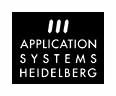
\includegraphics[width=0.5\linewidth]{img/ash}}

\maketitle

\begin{abstract}
    In the 1980s, when personal computers with graphical user interfaces
    began to become common in homes and universities, there was an increasing demand to use computers to help with document preparation.
    
    Sometimes referred to as the \textit{\acrfull{dtp} revolution}, this decade saw the invention of \acrshort{dtp} technology that set the foundation for the tools we use today. This includes the initial releases of WordStar (1978), Microsoft Word (1983), PostScript (1984), \TeX{} (1986), and PDF (1993).
    
    This paper describes one of the tools of the time. The \gls{Signum!2} word processing system was a common tool used to write theses and papers in Germany in the 1980s. It was only available on the ATARI ST line of personal computers, created by mathematician Franz Schmerbeck and published by \acrfull{ash}.
    
    \Signum{} was never released for newer operating systems after the ATARI ST was discontinued. The documents that were prepared with it are not compatible with modern software and conversions to other formats are rare and incomplete. In this paper, I also present the results of my personal research into these files, the approach that I took and what I learned about the way \Signum{} works.
\end{abstract}

\tableofcontents

\section*{Introduction}
\label{sec:intro}
\addcontentsline{toc}{section}{\nameref{sec:intro}}

%\fixme{Sachlicher}
% - This is what I did
% - "Contributions"
% - Explain what Signum! is relative to ATARI
% - Why now -- missing experience 10 years ago

This paper describes my experience with extracting text documents from a discontinued computer system – from reading files off of floppy disks that were stored in my parents' basement to decoding images in an undocumented file format.

I provide a short overview over the ATARI ST line of computers, the components that it consists of and available methods to use its programs and storage devices in the present day. Then, I present the commercial \Signum{} word processing system, its motivation, mechanics and basic user interface.

Next, I present general concepts of file formats and original research into two file formats that are used by Signum. This is information that was not previously available to the public.

Finally, I provide an overview of existing methods to convert Signum documents into more modern formats, introduce my own system to convert Signum files to \acrshort{pdf} and discuss key challenges and decisions pertaining to that project.

%In August of 2020, I started to look into a box of old floppy disks from my parents' basement. These disks were originally used on an ATARI ST and later a Windows 95 machine, that are still stored in the same room.

%A few of the disks were marked with the term \textit{Signum!}. My dad told me that this was the program he used to write his masters thesis (\textit{Magister Artium}) and that the thesis itself should be on one of the disks as well.

%So, after making copies of all the floppy disks that were still in good shape, I focused on the ones that were related to Signum!. I was very excited to find files like \textbf{EINLEITU.SDO}, \textbf{MAGISTER.SDO} and \textbf{SCHLUSS.SDO} on one of the disks, but also realized that this was a custom file format with no modern tools available to read it.

%Looking at the content of the files, I noticed that much of the text was actually readable with a bit of effort (c.f. \autoref{fig:sdo-hexdump}), so started to work on a system that automated this. In this process, I learned a lot about Signum!, it's file format and also word processing, document preparation and font handling in general, which is presented in this paper.

\paragraph{Contributions} This paper offers a description of the structure of the Signum!2 document file format, a description of the associated \textit{bimc} image file format and its compression algorithm and a description of three particular challenges that arise from creating a new software that reads those files, namely character positioning, using bitmap fonts and character encoding.